\ifx\allfiles\undefined
\documentclass[12pt, a4paper, oneside, UTF8]{ctexbook}
\def\path{../config}
\usepackage{amsmath}
\usepackage{amsthm}
\usepackage{amssymb}
\usepackage{graphicx}
\usepackage{mathrsfs}
\usepackage{enumitem}
\usepackage{geometry}
\usepackage[colorlinks, linkcolor=black]{hyperref}
\usepackage{stackengine}
\usepackage{yhmath}
\usepackage{extarrows}

\usepackage{multicol}
\usepackage{fancyhdr}
\usepackage[dvipsnames, svgnames]{xcolor}
\usepackage{listings}
\usepackage{subfigure}
\usepackage{tikz}


\definecolor{mygreen}{rgb}{0,0.6,0}
\definecolor{mygray}{rgb}{0.5,0.5,0.5}
\definecolor{mymauve}{rgb}{0.58,0,0.82}

\graphicspath{ {figure/},{../figure/}, {config/}, {../config/} }

\linespread{1.6}

\geometry{
    top=25.4mm, 
    bottom=25.4mm, 
    left=20mm, 
    right=20mm, 
    headheight=2.17cm, 
    headsep=4mm, 
    footskip=12mm
}

\setenumerate[1]{itemsep=5pt,partopsep=0pt,parsep=\parskip,topsep=5pt}
\setitemize[1]{itemsep=5pt,partopsep=0pt,parsep=\parskip,topsep=5pt}
\setdescription{leftmargin=4em,itemsep=5pt,partopsep=0pt,parsep=\parskip,topsep=5pt}

\lstset{
    language=Mathematica,
    basicstyle=\tt,
    breaklines=true,
    keywordstyle=\bfseries\color{NavyBlue}, 
    emphstyle=\bfseries\color{Rhodamine},
    commentstyle=\itshape\color{black!50!white}, 
    stringstyle=\bfseries\color{PineGreen!90!black},
    columns=flexible,
    numbers=left,
    numberstyle=\footnotesize,
    frame=tb,
    breakatwhitespace=false,
} 
% 定理环境
\usepackage{tcolorbox}
\tcbuselibrary{most}
\theoremstyle{definition}


\newtheorem{proposition}{\indent 命题}[section]
\newtheorem{example}{\indent \color{SeaGreen}{例}}[section]
\theoremstyle{plain}
\newtheorem*{rmk}{\indent 注}
\renewenvironment{proof}{\indent\textcolor{SkyBlue}{\textbf{证明.}}\;}{\qed\par}
\newenvironment{solution}{\indent\textcolor{SkyBlue}{\textbf{解.}}\;}{\qed\par}
% #### 将 config.tex 中的定理环境的对应部分替换为如下内容
% 定义单独编号,其他四个共用一个编号计数 这里只列举了五种,其他可类似定义(未定义的使用原来的也可)
\newtcbtheorem[number within=section]{defn}%
{定义}{colback=OliveGreen!10,colframe=Green!70,fonttitle=\bfseries}{def}

\newtcbtheorem[number within=section]{lemma}%
{引理}{colback=Salmon!20,colframe=Salmon!90!Black,fonttitle=\bfseries}{lem}

% 使用另一个计数器 use counter from=lemma
\newtcbtheorem[use counter from=lemma, number within=section]{them}%
{定理}{colback=SeaGreen!10!CornflowerBlue!10,colframe=RoyalPurple!55!Aquamarine!100!,fonttitle=\bfseries}{them}

\newtcbtheorem[use counter from=lemma, number within=section]{criterion}%
{准则}{colback=green!5,colframe=green!35!black,fonttitle=\bfseries}{cri}

\newtcbtheorem[use counter from=lemma, number within=section]{corollary}%
{推论}{colback=Emerald!10,colframe=cyan!40!black,fonttitle=\bfseries}{cor}
% colback=red!5,colframe=red!75!black

% 这个颜色我不喜欢
%\newtcbtheorem[number within=section]{proposition}%
%{命题}{colback=red!5,colframe=red!75!black,fonttitle=\bfseries}{cor}

% .... 命题 例 注 证明 解 使用之前的就可以(全文都是这种框框就很丑了),也可以按照上述定义 ...
\def\d{\mathrm{d}}
\def\R{\mathbb{R}}
\def\C{\mathbb{C}}
\def\a{\bs{a}}
\def\b{\bs{b}}
\def\x{\bs{x}}
\def\y{\bs{y}}
\def\z{\bs{z}}
\def\u{\bs{u}}
\def\A{\bs{A}}
\def\B{\bs{B}}
\def\D{\bs{D}}
\def\G{\bs{G}}
\def\H{\bs{H}}
\def\L{\bs{L}}
\def\Q{\bs{Q}}
\def\X{\bs{X}}
\def\Y{\bs{Y}}
\def\Z{\bs{Z}}
\def\U{\bs{U}}
\def\V{\bs{V}}
\def\P{\bs{P}}
\def\J{\bs{J}}
\def\I{\bs{I}}
\def\E{\bs{E}}
\newcommand{\bs}[1]{\boldsymbol{#1}}
\newcommand{\ora}[1]{\overrightarrow{#1}}
\newcommand{\myspace}[1]{\par\vspace{#1\baselineskip}}
\newcommand{\xrowht}[2][0]{\addstackgap[.5\dimexpr#2\relax]{\vphantom{#1}}}
\newenvironment{ca}[1][1]{\linespread{#1} \selectfont \begin{cases}}{\end{cases}}
\newenvironment{vx}[1][1]{\linespread{#1} \selectfont \begin{vmatrix}}{\end{vmatrix}}
\newcommand{\tabincell}[2]{\begin{tabular}{@{}#1@{}}#2\end{tabular}}
\newcommand{\pll}{\kern 0.56em/\kern -0.8em /\kern 0.56em}
\newcommand{\dive}[1][F]{\mathrm{div}\;\bs{#1}}
\newcommand{\rotn}[1][A]{\mathrm{rot}\;\bs{#1}}
\newcommand{\rank}{\text{rank}}

\def\myIndex{0}
% \input{\path/cover_package_\myIndex.tex}

\def\myTitle{矩阵理论复习笔记}
\def\myAuthor{}
\def\myDateCover{}
\def\myDateForeword{\\\today}
\def\myForeword{前言}
\def\myForewordText{\par
本复习笔记是我个人在学习矩阵理论的过程中整理、总结而成,包含课本的内容、上课PPT涉及到的内容以及不懂地方的补充知识,希望能够对你有所帮助。\par 全书排版是利用\LaTeX 完成的,这也是对我使用\LaTeX 的一次较大工程的练手,希望我能在撰写完之后对于\LaTeX 使用有更深层次的理解。\par 因本人水平有限,故本总结笔记如有不当之处,敬请指出,本人不胜感激!
}
\def\mySubheading{}


\begin{document}
\input{\path/cover_text_\myIndex.tex}

\newpage
\thispagestyle{empty}
\begin{center}
    \Huge\textbf{\myForeword}
\end{center}
\myForewordText
\begin{flushright}
    \begin{tabular}{c}
        \myDateForeword
    \end{tabular}
\end{flushright}

\newpage
\pagestyle{plain}
\setcounter{page}{1}
\pagenumbering{Roman}
\tableofcontents

\newpage
\pagenumbering{arabic}
\setcounter{chapter}{-1}
\setcounter{page}{1}

\pagestyle{fancy}
\fancyfoot[C]{\thepage}
\renewcommand{\headrulewidth}{0.4pt}
\renewcommand{\footrulewidth}{0pt}








\else
\fi
\chapter{线性代数基本知识}
本章主要针对矩阵理论中所涉及到的线性代数知识进行复习与回顾,随着课程的进行,当认为有必要需要补充相关的线性代数基本知识时,会补充在本节。

本章会涉及以下内容:

\begin{itemize}[leftmargin=4em]
    \item 行列式
    \item 矩阵
    \item 向量组、线性方程组
    \item 特征值与特征向量,矩阵相似理论
\end{itemize}
\textbf{注意:}本章只作为一个对于基本知识的回顾与复习,并不会涉及到更详细的解释,如果需要查看更详细的解释,请翻阅对应的线性代数教材或上网搜集资料。
\footnote{本章的大多数内容是在《2025张宇考研数学基础30讲——线性代数分册》的基础上整理总(抄)结(写)而成}
\newpage
\section{行列式}

行列式作为后续矩阵理论中涉及特征值与特征向量计算的基础,因此有必要复习巩固行列式的定义、行列式的相关性质以及具体行列式的计算。
\subsection{行列式的定义与计算方法}
何为行列式?如果查阅线性代数的教材(这里以同济六版《线性代数》为例),会发现教材是从特例到一般进行推广,首先给出二阶行列式和三阶行列式应如何计算,后面给出全排列的逆序数的概念,最后推广至$n$阶行列式得出$n$阶行列式的定义的,而在介绍二阶行列式的时候,是先从解一个二元线性方程组得出的:
\begin{figure}[h]
    \centering
    \subfigure[教材中对于二阶行列式的介绍]{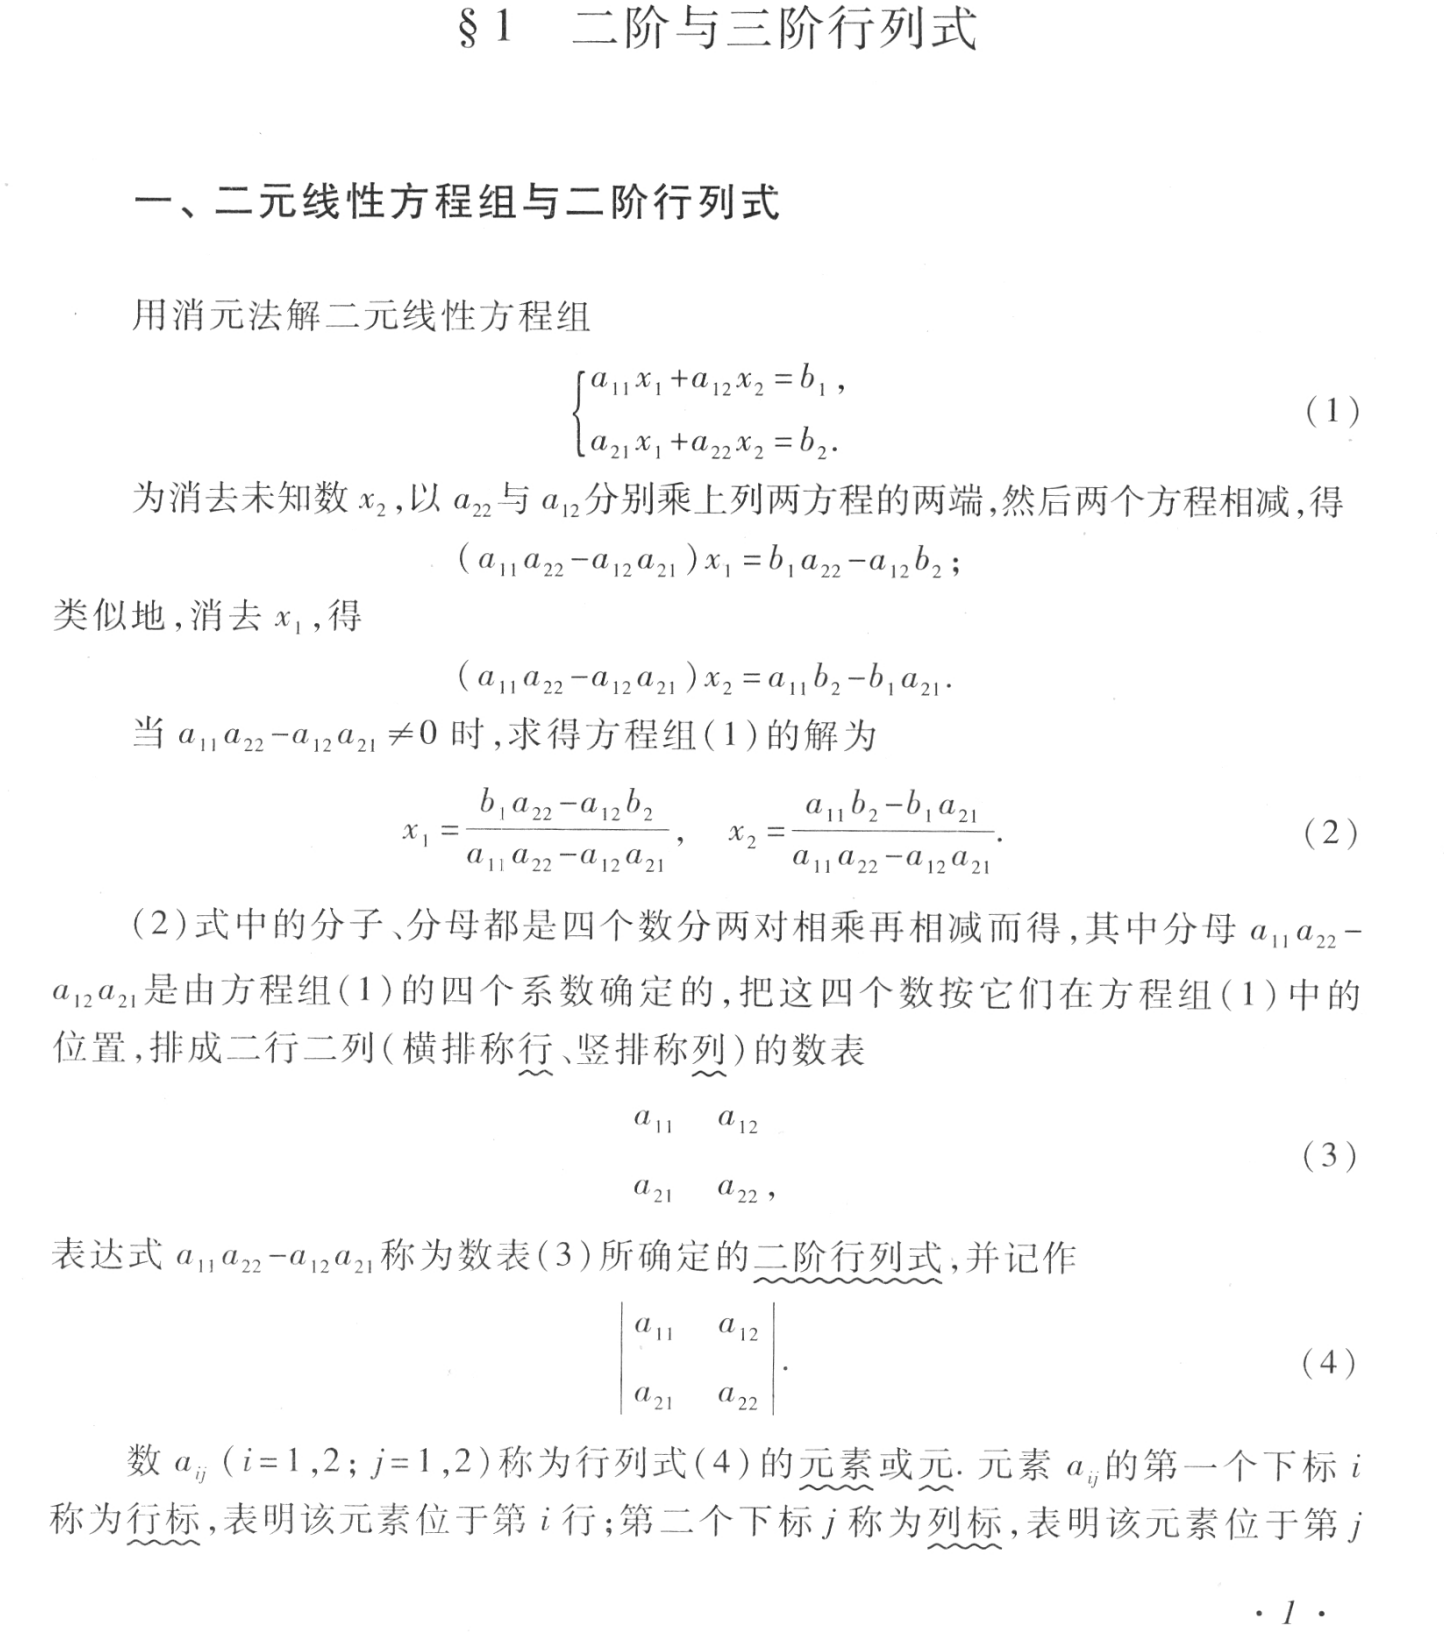
\includegraphics[scale=0.3]{../figure/行列式.png}}
    \subfigure[教材中对于二三行列式的介绍]{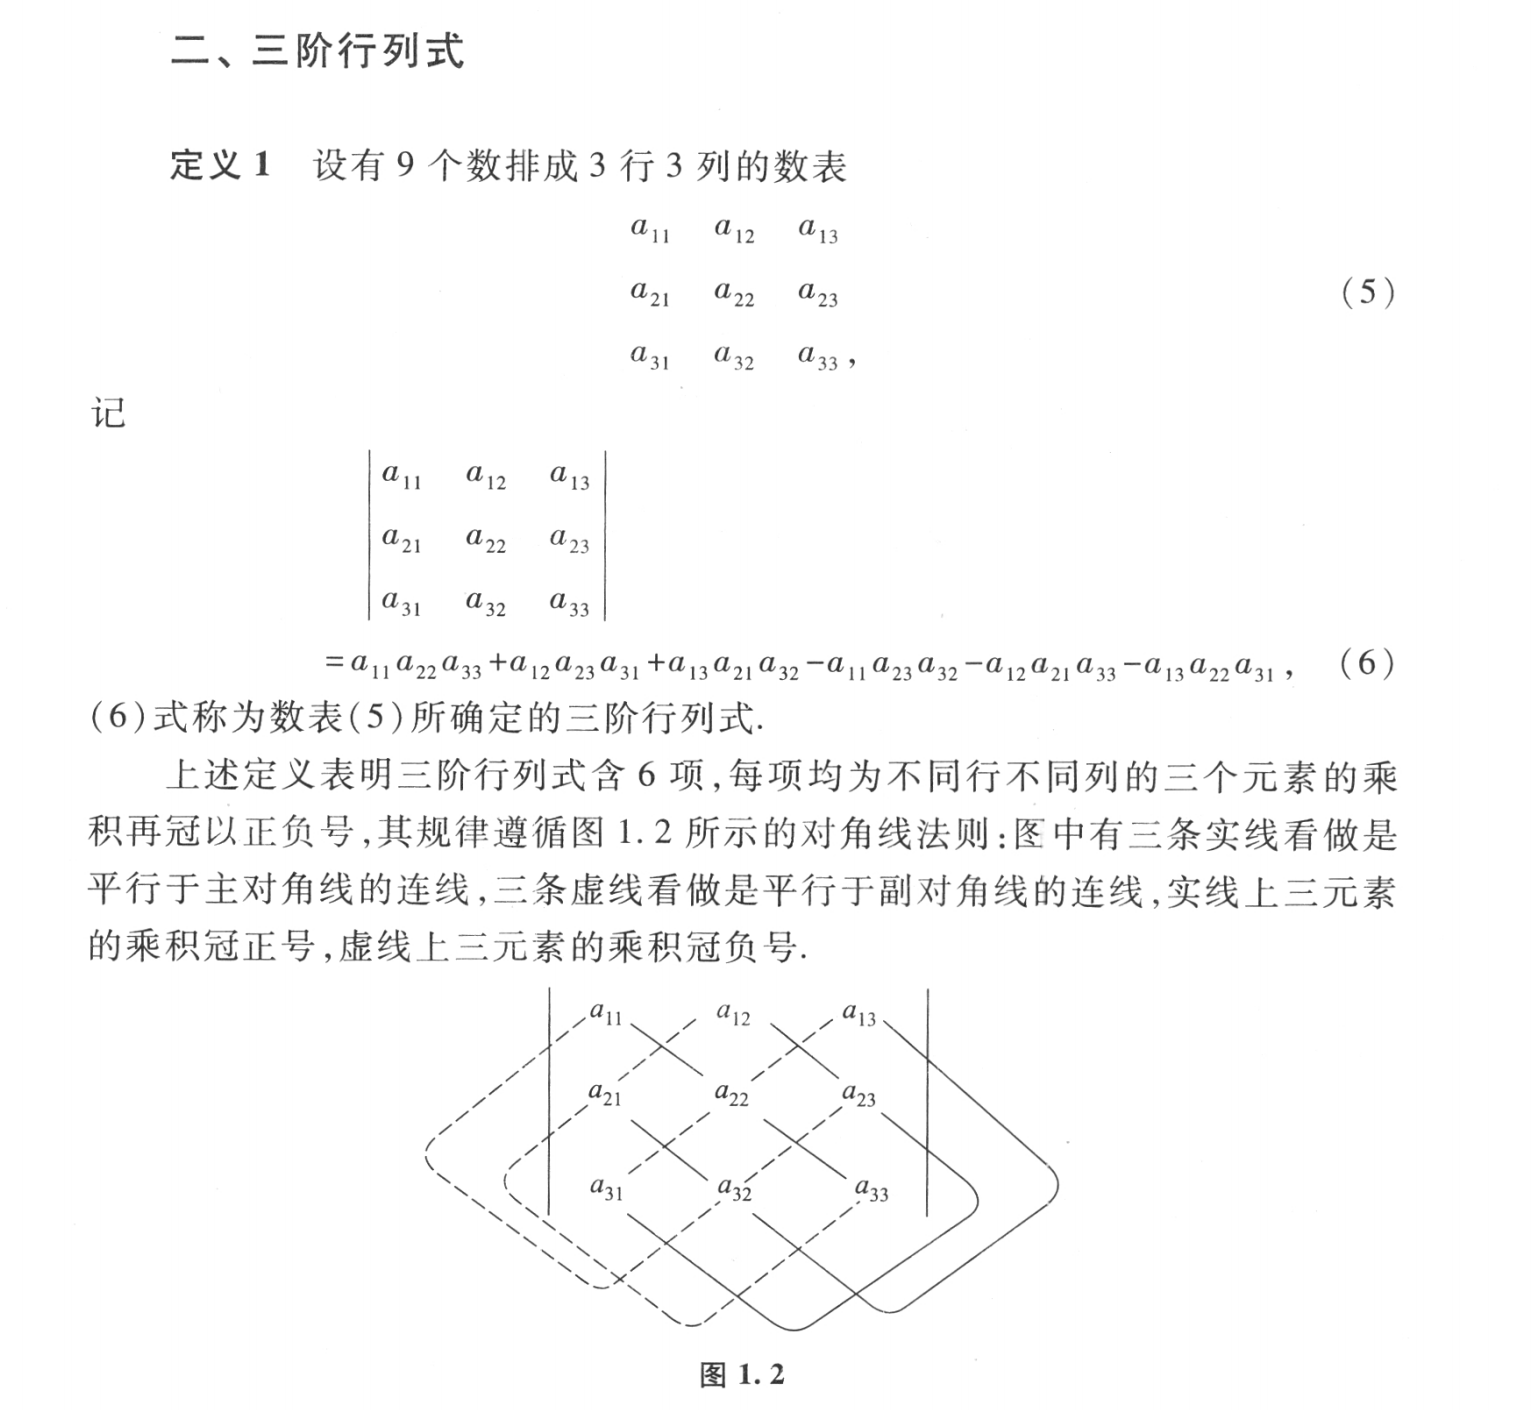
\includegraphics[scale=0.3]{../figure/行列式2.png}}
    \caption{《线性代数》教材中对于二阶、三阶行列式的介绍}
\end{figure}

这样的定义是从代数的角度出发的,可能对于行列式的理解并不是很清楚,接下来会给出除课本之外的另一种理解行列式的方法。
\subsubsection{行列式的第一种定义}
假设我们有如下的一个二阶行列式:
\[
    \begin{vmatrix}
    a_{11} & a_{12}\\
    a_{21} & a_{22}
    \end{vmatrix}
\]

我们将该行列式的第一行看作一个向量, 即$\bs {a_1}=\left[a_{11}, a_{12}\right]$, 将第二行看作另外一个向量,即$\bs {a_2}=\left[a_{21}, a_{22}\right]$, 将这两个向量放在平面直角坐标系中,并以这两条边构建成一个平行四边形,如下图所示:

\begin{figure}[htbp]
    \centering
    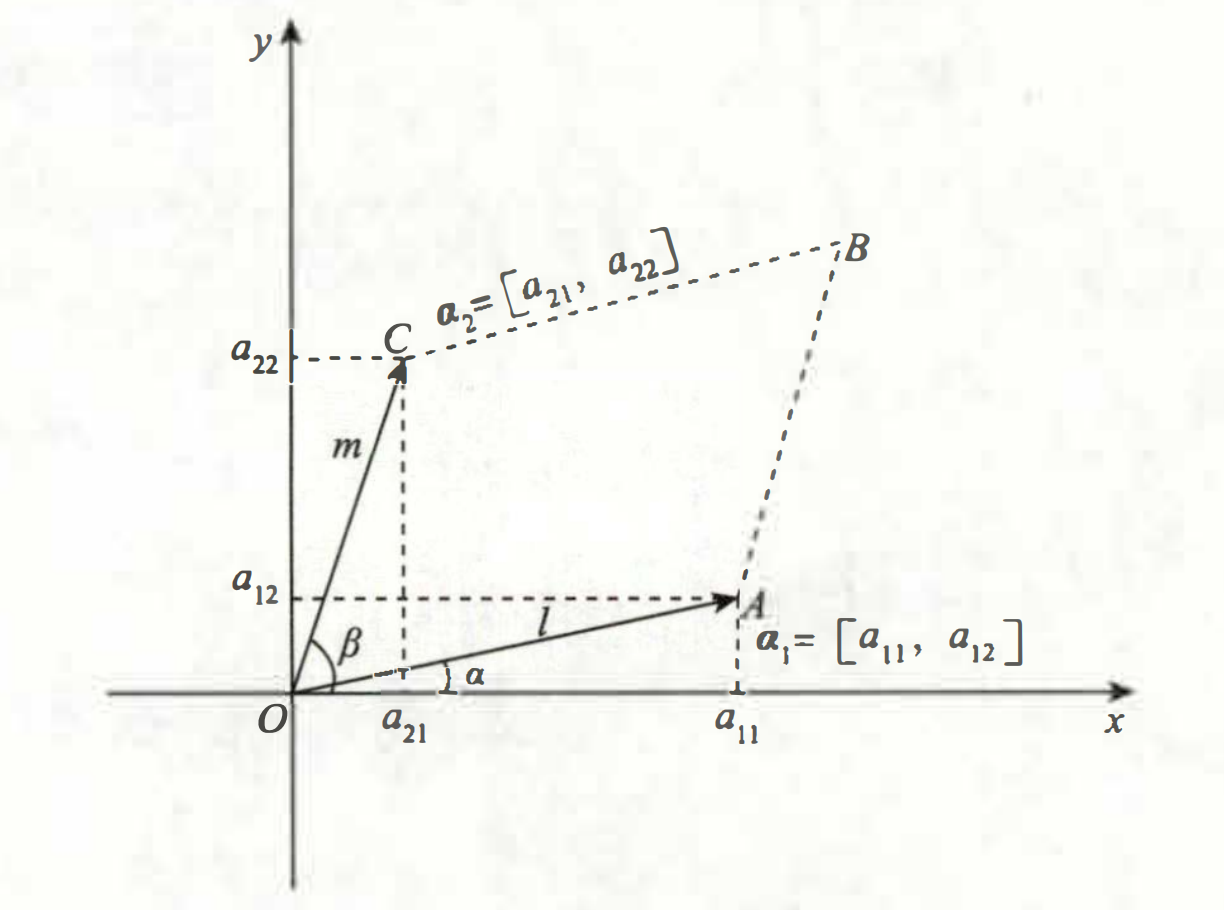
\includegraphics[scale=0.5]{../figure/平行四边形.png}
    \caption{将两个向量放在平面直角坐标系中表示的效果图}
\end{figure}

那么,这个平行四边形的面积是多少呢?我们设$\bs{a_1}$与$x$轴的夹角为$\alpha$, $\bs{a_2}$与$x$轴的夹角为$\beta$, 设$||\bs{a_1}|| = l, ||\bs{a_2}|| = m$。

则,平行四边形的面积为:
\[
  \begin{aligned}
    S &= l\cdot m\cdot\sin(\beta-\alpha)\\
    &= l\cdot m(\sin\beta\cos\alpha-\cos\beta\sin\alpha)\\
    &= l\cos\alpha\cdot m\sin\beta-l\sin\alpha\cdot\cos\beta\\
    &= a_{11}a_{22} - a_{12}a_{21}
  \end{aligned}  
\]

这是不是与二阶行列式的结果一样呢?所以我们可以得出一个结论:二阶行列式可以表示为一个平行四边形的面积。
\newpage
接下来我们讨论三阶行列式,与二阶行列式相似,假设我们有如下三阶行列式:
\[
    \begin{vmatrix}
      a_{11} & a_{12} & a_{13}\\
      a_{21} & a_{22} & a_{23}\\
      a_{31} & a_{32} & a_{33}      
    \end{vmatrix}
\]

其实,三阶行列式的几何意义即为是一个由三个三维向量$\bs{a_1}=\left[a_{11}, a_{12}, a_{13}\right], \bs{a_2}=[a_{21}, a_{22},$\\$ a_{23}], \bs{a_3}=\left[a_{31}, a_{32}, a_{33}\right]$组成的一个平行六面体的体积,如下图:
\begin{figure}[htbp]
    \centering
    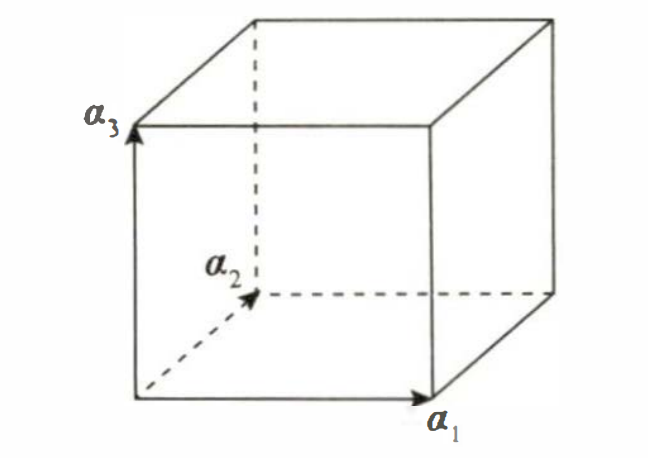
\includegraphics[scale=0.5]{../figure/平行六面体.png}
    \caption{三阶行列式的几何意义示意}
\end{figure}

再进行推广,我们可以得到$n$阶行列式的定义:

\begin{defn}{}{}
一个$n$阶行列式
\[D_n=
    \begin{vmatrix}
      a_{11} & \cdots & a_{1n}\\
      \vdots & & \vdots\\
      a_{1n} & \cdots & a_{nn}  
    \end{vmatrix}    
\]
其是由$n$个$n$维向量:
\[
    \begin{aligned}
    \bs{a_1}&=\left[a_{11}, a_{12}, \cdots, a_{1n}\right]\\
    \bs{a_2}&=\left[a_{21}, a_{22}, \cdots, a_{2n}\right]\\
    &\dots\\
    \bs{a_n}&=\left[a_{n1}, a_{n2}, \cdots, a_{nn}\right]
    \end{aligned} 
\]
组成的,其结果是以这$n$个向量为边的$n$维图形的“体积”。
\end{defn}

这里可以结合后面线性相关和线性无关的性质:如果一个方阵的行列式为$0$,就说这个向量组是线性相关的,如果用行列式的几何意义理解将会变得十分简单,因为如果一个向量组线性相关,就说明这个向量组至少有一个向量是与其他的向量共线的,如果共线,就说明这个$n$维图形将会少一条边,少一条边“体积”自然为0。
\subsubsection{行列式的第二种定义}
后面行列式的第二种与第三种定义与教材中对于行列式的定义相同,第二种行列式引入了“逆序数”这一概念来辅助定义行列式,即一个$n$阶行列式:
\[
    \begin{vmatrix}
        a_{11} & \cdots & a_{1n}\\
        \vdots & & \vdots\\
        a_{1n} & \cdots & a_{nn}  
      \end{vmatrix}   
=\sum_{j_1j_2\cdots j_n}(-1)^{r(j_1j_2\cdots j_n)}a_{1j_1}a_{2j_2}\cdots a_{nj_n}
\]
这里$r(j_1j_2\cdots j_n)$表示的是数列$j_1,j_2,\cdots,j_n$的逆序数\footnote{关于逆序数的详细解释,请参阅: \url{https://zhuanlan.zhihu.com/p/398845457}}。

\begin{rmk}
    如何理解上面的公式:计算一个$n$阶行列式只需要找出其所有的行和所有的列的展开乘以对应的系数($-1$的正负),最后将所有的和加起来即为行列式的值。
\end{rmk}

\subsubsection{行列式的第三种定义}
这里介绍行列式的第三种定义——代数余子式与余子式形式,这一种定义也是计算行列式的常用方法。

首先,回顾一下什么是余子式,什么是代数余子式:
\begin{itemize}
    \item 余子式:将一个$n$阶行列式,去掉元素$a_{ij}$所在的行和列(即第$i$行和第$j$列)之后得到的新的行列式,记为$\bs{M_{ij}}$。
    \item 代数余子式:余子式乘以$(-1)^{i+j}$记为代数余子式,记为$\bs{A_{ij}}$。
\end{itemize}

根据上面的介绍,不难得出下列关系:
\[A_{ij}=(-1)^{i+j}M_{ij}\]

由此,可以得出行列式的第三种定义:
\begin{defn}{}{}
    可以按照某一行某一列来展开行列式,即:
    \[|\bs{A}| =
        \begin{cases}
            a_{i1}A_{i1}+a_{i2}A_{i2}+\cdots+a_{in}A_{in}=\sum\limits_{j=1}^{n}a_{ij}A_{ij}&(i=1,2,\cdots,n)\rightarrow(\text{按行展开})\\
            a_{1j}A_{1j}+a_{2j}A_{2j}+\cdots+a_{nj}A_{nj}=\sum\limits_{i=1}^{n}a_{ij}A_{ij}&(j=1,2,\cdots,n)\rightarrow(\text{按列展开})
        \end{cases}    
    \]
\end{defn}

\begin{rmk}
    行列式的某一行或者某一列乘以其他非对应行或非对应列的代数余子式后再求和,其结果为$0$。
\end{rmk}
\begin{example}
    试计算行列式\[
        D=
        \begin{vmatrix}
            2&-1&0&0\\
            0&2&-1&0\\
            0&0&2&-1\\
            -1&0&0&2
        \end{vmatrix}
        \]
\end{example}
\begin{solution}
    计算行列式的值,按照定义三来解题的话,尽可能找“$0$”多的行或者列进行展开,这样可以简单计算。

    将行列式按第一列展开,得
    
    \[
         \begin{aligned}
            D&=2\begin{vmatrix}
                2&-1&0\\
                0&2&-1\\
                0&0&2
            \end{vmatrix}
            -1\times(-1)^{(4+1)}\begin{vmatrix}
                -1&0&0\\
                2&-1&0\\
                0&2&-1
            \end{vmatrix}\\
            &=16-1=15
         \end{aligned}
    \]
\end{solution}
\subsection{行列式的性质}
只知道了行列式的计算还不够,运用好行列式的性质可以在处理复杂行列式的时候及时发现其规律对其进行处理,从而达到简便计算的效果。

行列式有下列性质:
%\setlist[description]{labelsep=1em, leftmargin=2em}
\begin{itemize}[leftmargin=4em]
    \item 行列互换,其值不变,即$|\bs{A}|=|\bs{A}^{T}|$
    \item 若行列式中的某一行或者某一列的元素全为$0$,则行列式为$0$
    \item 若行列式中某一行或者某一列有公因子$k(k\neq0)$,则可以将该公因子提到行列式外面,即:
    \[
    \begin{vmatrix}
        a_{11}&a_{12}&\cdots&a_{1n}\\
        \vdots&\vdots&&\vdots\\
        ka_{11}&ka_{12}&\cdots&ka_{1n}\\
        \vdots&\vdots&&\vdots\\
        a_{n1}&a_{n2}&\cdots&a_{1nn}
    \end{vmatrix}=
    \begin{vmatrix}
        ka_{11}&a_{12}&\cdots&a_{1n}\\
        \vdots&\vdots&&\vdots\\
        ka_{11}&a_{12}&\cdots&a_{1n}\\
        \vdots&\vdots&&\vdots\\
        ka_{n1}&a_{n2}&\cdots&a_{1nn}
    \end{vmatrix}=k
    \begin{vmatrix}
        a_{11}&a_{12}&\cdots&a_{1n}\\
        \vdots&\vdots&&\vdots\\
        a_{11}&a_{12}&\cdots&a_{1n}\\
        \vdots&\vdots&&\vdots\\
        a_{n1}&a_{n2}&\cdots&a_{1nn}
    \end{vmatrix}
    \]
    \begin{rmk}
        ~
        \begin{enumerate}
            \item 这叫做行列式的“倍乘”性质
            \item 请注意在行列式中可以提出公因子和矩阵里可以提出公因子的区别,在矩阵中需要要求所有所有元素都含有公因子才可以提出来。
        \end{enumerate}
    \end{rmk}
    \item 行列式中某一行或者某一列的元素均是某两个数之和,则可以将行列式拆成两个行列式之和,即
    \[\begin{vmatrix}
        a_{11} & a_{12} & \cdots & a_{1n}\\
        \vdots & \vdots &  & \vdots\\
        a_{i1}+b_{i1} & a_{i2}+b_{i2} &\cdots & a_{in} + b_{in}\\
        \vdots & \vdots &  & \vdots\\
        a_{n1} & a_{n2} & \cdots & a_{nn}
    \end{vmatrix}=
    \begin{vmatrix}
        a_{11} & a_{12} & \cdots & a_{1n}\\
        \vdots & \vdots &  & \vdots\\
        a_{i1} & a_{i2} &\cdots & a_{in}\\
        \vdots & \vdots &  & \vdots\\
        a_{n1} & a_{n2} & \cdots & a_{nn}
    \end{vmatrix}+
    \begin{vmatrix}
        a_{11} & a_{12} & \cdots & a_{1n}\\
        \vdots & \vdots &  & \vdots\\
        b_{i1} & b_{i2} &\cdots & b_{in}\\
        \vdots & \vdots &  & \vdots\\
        a_{n1} & a_{n2} & \cdots & a_{nn}
    \end{vmatrix}
    \]
    \begin{rmk}
        请仔细留意该性质成立的条件
    \end{rmk}
    \item 行列式中两行或两列互换,行列式变号
    \item 行列式中两行或两列的元素对应成比例,则行列式结果为$0$
    \item 行列式中的某一行或某一列的$k$倍加到另外一行或另外一列,行列式不变
    \begin{rmk}
        这也叫行列式的倍加性质
    \end{rmk}
\end{itemize}
\begin{rmk}
    以上的性质可以结合行列式的几何意义辅助理解
\end{rmk}
\begin{example}
    设关于$\lambda$的方程
    \[
        \begin{vmatrix}
            \lambda-1&-2&3\\
            1&\lambda-4&3\\
            -1&a&\lambda-5
        \end{vmatrix}=0
    \]
    有二重根,求$a$的值
\end{example}
\begin{solution}
    将行列式的第一行与第二行相减,得\[
        \begin{vmatrix}
            \lambda-2&2-\lambda&0\\
            1&\lambda-4&3\\
            -1&a&\lambda-5
        \end{vmatrix}
    \]
    将行列式的第一列加到第二列,得\[
        \begin{vmatrix}
            \lambda-2&0&0\\
            1&\lambda-3&3\\
            -1&a-1&\lambda-5
        \end{vmatrix}
    \]
    按第一行展开,有\[
        \begin{aligned}(\lambda-2)
        \begin{vmatrix}
            \lambda-3&3\\
            a-1&\lambda-5
        \end{vmatrix}&=(\lambda-2)[(\lambda-3)(\lambda-5)-3(a-1)]\\
        &=(\lambda-2)(\lambda^2-8\lambda+18-3a)=0
    \end{aligned}
    \]
    若想让函数有一个二重根,则需要满足$\lambda^2-8\lambda+18-3a$有二重根。

    由求根公式得,$\triangle=-\frac{b^2-4ac}{2a}=(-8)^2-4(18-3a)=0$

    解得$a=\frac{2}{3}$
\end{solution}
\section{矩阵}
在介绍了行列式之后,本小节主要介绍矩阵的运算性质、矩阵的逆、矩阵的秩、一些特殊的矩阵,以及矩阵的初等变换等内容。
\subsection{矩阵的运算性质}
矩阵的运算性质如下:
\begin{itemize}[leftmargin=4em]
    \item 矩阵的加法: 对应项元素相加即可
    \item 矩阵的乘法:左边矩阵的每一行乘以右边矩阵的每一列,将求得的和写在对应位置,请注意矩阵乘法需要满足左侧矩阵的列与右侧矩阵的行相等才能进行
    \item 数乘矩阵:$k\bs{A}=\bs{A}k=k\begin{bmatrix}
        a_{11}&a_{12}&\cdots&a_{1n}\\
        a_{21}&a_{22}&\cdots&a_{2n}\\
        \vdots&\vdots&&\vdots\\
        a_{m1}&a_{m2}&\cdots&a_{mn}
    \end{bmatrix}=\begin{bmatrix}
        ka_{11}&ka_{12}&\cdots&ka_{1n}\\
        ka_{21}&ka_{22}&\cdots&ka_{2n}\\
        \vdots&\vdots&&\vdots\\
        ka_{m1}&ka_{m2}&\cdots&ka_{mn}
    \end{bmatrix}$
    \begin{rmk}
        注意这里与前面行列式倍乘性质的区别
    \end{rmk}
    \item 矩阵的加法满足交换律、结合律,矩阵的数乘满足分配律、交换律和结合律,\textbf{但矩阵之间的乘法只满足结合律和分配律,一般不满足交换律}
    \item 转置矩阵满足下面的运算律
    \begin{enumerate}
        \item $(\bs{A}^T)^T=A$
        \item $(k\bs{A})^T=k\bs{A}^T$
        \item $(\bs{A+B})^T=\bs{A}^T+\bs{B}^T$
        \item $(\bs{A}\bs{B})^T=\bs{B}^T\bs{A}^T\rightarrow\text{“穿脱原则”}$
    \end{enumerate}
\end{itemize}
\subsection{矩阵的逆}
\begin{defn}{逆矩阵定义}{}
    设$\bs{A}, \bs{B}$是$n$阶方阵,$E$是$n$阶单位矩阵,若$\bs{AB=BA=E}$,则称$\bs{A}$是可逆矩阵,$\bs{B}$是$\bs{A}$的逆矩阵,记为$\bs{A}^{-1}$。
\end{defn}
\begin{rmk}
    $\bs{A}$矩阵可逆的充要条件是$|\bs{A}|\neq0$。
\end{rmk}
\subsubsection{逆矩阵的性质与重要公式}
设$\bs{A, B}$为同阶可逆矩阵,则
\begin{enumerate}[leftmargin=4em]
    \item $(\bs{A}^{-1})^{-1}=\bs{A}$
    \item 若$k\neq0$,则$(k\bs{A})^{-1}=\frac{1}{k} \bs{A}^{-1}$
    \item $\bs{AB}$也可逆,则$(\bs{AB})^{-1}=\bs{B}^{-1}\bs{A}^{-1}$
    \item $\bs{A}^T$也可逆,且$(\bs{A}^T)^{-1}=(\bs{A}^{-1})^{T}$
    \item $|\bs{A}^{-1}|=|\bs{A}|^{-1}$
\end{enumerate}
\begin{rmk}
    $\bs{A+B}$不一定可逆,且$(\bs{A+B})^{-1}\neq\bs{A}^{-1}+\bs{B}^{-1}$
\end{rmk}
\subsection{矩阵的伴随}
\subsubsection{伴随矩阵的定义}
\begin{defn}{}{}
    \[
        A^*=\begin{bmatrix}
            A_{11} & A_{21} & \cdots & A_{n1}\\
            A_{12} & A_{22} &  \cdots & A_{n2}\\
            \vdots & \vdots &  & \vdots\\
            A_{1n} & A_{2n} & \cdots & A_{nn}
        \end{bmatrix}
    \]
    其中$A_{ij}$代表代数余子式。
\end{defn}
\subsubsection{伴随矩阵的性质与重要公式}
伴随矩阵具有下列的性质:
\begin{itemize}[leftmargin=4em]
    \item 对任意$n$阶方阵$\bs{A}$,都有伴随矩阵$\bs{A}^*$,且有公式\[\bs{AA^*}=\bs{A^*A}=|\bs{A}|\bs{E}\]\[|\bs{A}|^*=|\bs{A}|^{n-1}\]
\end{itemize}

当$|\bs{A}|\neq0$的时候,有
\begin{multicols}{2}
\begin{itemize}[leftmargin=4em]
    \item $\bs{A^*}=|\bs{A}|\bs{A}^{-1}$
    \item $\bs{A}^{-1}=\frac{1}{|\bs{A|}}\bs{A}^*$
    \item $\bs{A}=|\bs{A}| ({\bs{A}}^*)^{-1}$
    \item $ (k\bs{A}) (k\bs{A})^*=|k\bs{A}|\bs{E}$
    \item $\bs{A}^T (\bs{A}^T)^*=|\bs{A}^T|\bs{E}$
    \item $\bs{A}^{-1} (\bs{A}^{-1})^*=|\bs{A}^{-1}|\bs{E}$
    \item $\bs{A}^* (\bs{A}^*)^*=|\bs{A}^*|\bs{E}$
    \item $ (\bs{A}^T)^*= (\bs{A}^*)^T$
    \item $ (\bs{A}^{-1})^*= (\bs{A}^*)^{-1}$
    \item $ (\bs{AB})^*=\bs{B}^*\bs{A}^*$
    \item $ (\bs{A}^*)^*=|\bs{A}|^{n-2}\bs{A}$
\end{itemize}
\end{multicols}
\begin{rmk}
    $ (\bs{A+B}^*)\neq\bs{A}^*+\bs{B}^*$
\end{rmk}
\subsection{初等矩阵与初等变换}
\subsubsection{初等变换}
有如下三种初等变换:
\begin{enumerate}[leftmargin=4em]
    \item 一个非零常数乘矩阵的某一行或某一列\ $\rightarrow$ 倍乘性质
    \item 矩阵中的某两行或两列互换位置\ $\rightarrow$ 互换性质
    \item 将某一行或某一列的$k$倍加到另外一行或另外一列中\ $\rightarrow$倍加性质
\end{enumerate}

以上三种变换叫做\textbf{初等行变换/初等列变换}
\subsubsection{初等矩阵}
由单位矩阵经过一次初等变换得到的矩阵叫做初等矩阵以三阶矩阵为例,有如下三种初等矩阵:
\begin{enumerate}[leftmargin=4em]
    \item $E_2(k)=\begin{bmatrix}
        1&0&0\\0&k&0\\0&0&1
    \end{bmatrix}$, $\bs{E}$的第2行或第2列乘$k$倍,称为倍乘初等矩阵
    \item $E_{12}=\begin{bmatrix}
        0&1&0\\1&0&0\\0&0&1
    \end{bmatrix}$, $\bs{E}$的第1,2行或第1,2列互换,称为互换初等矩阵
    \item $E_{31} (k)=\begin{bmatrix}
        1&0&0\\0&1&0\\k&0&1
    \end{bmatrix}$, $\bs{E}$的第1行的$k$倍加到第3行,或第3列的$k$倍加到第1列,称为倍加初等矩阵
\end{enumerate}

\subsubsection{行阶梯型矩阵和行最简阶梯型矩阵}
具有如下特性的矩阵称为\textbf{行阶梯形矩阵}:
\begin{itemize}[leftmargin=4em]
    \item 若有零行,必位于非零行的下方
    \item 各个非零行左起第一个非零元素的列标从上到下是严格增大的
\end{itemize}

当每一非零行的第一个元素为1,并且这些非零元素所在列的其他元素均为0,则这个矩阵就变成了\textbf{最简行阶梯型矩阵}.

\subsubsection{用初等变换求逆矩阵}
\begin{center}
    \[
        \begin{bmatrix}
        \bs{A}\vdots\bs{E}
        \end{bmatrix}
        \xrightarrow[]{\text{初等行变换}}
        \begin{bmatrix}
        \bs{E}\vdots\bs{A}^{-1}
        \end{bmatrix}
    \]

    \[
        \begin{bmatrix}
            \bs{A}\\\bs{E}
        \end{bmatrix}
        \xrightarrow[]{\text{初等列变换}}
        \begin{bmatrix}
            \bs{E}\\\bs{A}^{-1}
        \end{bmatrix}
    \]
\end{center}

\subsection{矩阵的秩}
矩阵的秩作为后续解线性方程组、向量组的关键性质,需要认真把握
\begin{defn}{矩阵的秩的定义}{}
    设$\bs{A}$是$m\times n$阶矩阵,若存在$k$阶子式(即,任取$k$行与$k$列构成的行列式)不为零,而任意$k+1$阶子式(如果有的话)全为0,则$r(\bs{A})=k$, 并且若$\bs{A}$为$n\times n$阶矩阵,则\[r(\bs{A})_{n\times n}=n\Leftrightarrow |\bs{A}|\neq0\Leftrightarrow\bs{A}\text{可逆}\]
\end{defn}

如果用定义求矩阵的秩较为麻烦,可以将行列式化成行阶梯型矩阵,其非零行的行数即为$\bs{A}$的秩.
\subsubsection{矩阵的秩的几个重要式子}
设$\bs{A}$是$m\times n$阶矩阵,$\bs{B}$是满足有关矩阵运算要求的矩阵,则:
\begin{itemize}[leftmargin=4em]
    \item $0\leq r(\bs{A})\leq \min{ \{m,n\}  }$
    \item $r(k\bs{A}) = r(\bs{A})(k\neq 0)$
    \item $r(\bs{AB}) \leq \min{\{r(\bs{A}, r(\bs{B}))\} }$
    \item $r(\bs{A+B})\leq r(\bs{A}) + r(\bs{B})$
    \item $r(\bs{A}^*)=\begin{cases}
        n,&r(\bs{A}=n)\\
        1,&r(\bs{A}=n-1)\\
        0,&r(\bs{A}<n-1)
    \end{cases}$
    \ \ \ \ 其中,$\bs{A}$为$n(n\geq2)$阶方阵
    \item 设$\bs{A}$为$m\times n$阶矩阵,$\bs{P,Q}$分别是$m,n$阶可逆矩阵,则\[r(\bs{A})=r(\bs{PA})=r(\bs{AQ})=r(\bs{PAQ})\]
    \item 若$\bs{A}_{m\times n}\bs{B}_{n\times s}=\bs{O}$, 则$r(\bs{A}+r(\bs{B})\leq n)$
    \item $r(\bs{A})=r(\bs{A}^T)=r(\bs{AA^T})=r(\bs{A^TA})$
\end{itemize}

关于矩阵的秩后续更详细介绍,请看向量组、线性方程组部分。
\section{矩阵的秩、向量组、线性方程组}
向量组与线性方程组的联系十分紧密,可以说这两个概念分别一个是从向量角度讨论,一个是在方程组的角度讨论,其本质是相同的,而在其中起重要作用的因子就是上一节最后介绍的矩阵的秩。
\subsection{向量以及向量组}
在本小节中,重点回顾向量组的线性相关、线性无关的概念及其相关性质。
\subsubsection{线性相关和线性无关}
\begin{defn}{线性相关}{}
    对于$m$个$n$维向量$a_1, a_2, \cdots, a_m$,若\textbf{存在}一组\textbf{不全为零}的数$k_1, k_2, \cdots, k_m$,使得\[k_1a_1+k_2a_2+\cdots+k_ma_m=0\]则称向量组$a_1,a_2,\cdots,a_m$\textbf{线性相关}.
\end{defn}
\begin{defn}{线性无关}{}
    若\textbf{不存在不全为零}的数$k_1, k_2, \cdots, k_m$,使得\[k_1a_1+k_2a_2+\cdots+k_ma_m=0\]则称向量组$a_1,a_2,\cdots,a_m$\textbf{线性无关},即,当且仅当$k_1=k_2=\cdots=k_n=0$的时候,才能使等式成立.
\end{defn}
\newpage
\subsubsection{判别线性相关性的几大定理}
\begin{enumerate}
    \item 向量组$a_1, a_2, \cdots, a_n(n\geq2)$线性相关的充要条件是向量组中至少有一个向量可以有其他的$n-1$个向量表示
    \begin{rmk}
        其逆否命题为:向量组$a_1, a_2, \cdots, a_n(n\geq2)$线性无关的充要条件是向量组中的任何一个向量都不能由其余的$n-1$个向量表示
    \end{rmk}
    \item 若向量组$a_1, a_2, \cdots, a_n$线性无关,而$\beta, a_1, a_2, \cdots, a_m$线性相关,则$\beta$可以由$a_1, a_2, \cdots, a_n$线性表示,且表示法唯一
    \item 如果向量组$\beta_1, \beta_2, \cdots, \beta_t$可以由向量组$a_1, a_2, \cdots, a_s$线性表示,且$t>s$, 则$\beta_1, \beta_2, \cdots, \beta_t$线性相关(以少表多,多的相关)
    \item 如果向量组$a_1, a_2, \cdots, a_m$有一部分向量线性相关,则整个向量组也线性相关
    \begin{rmk}
        其逆否命题为:如果向量组$a_1, a_2, \cdots, a_m$线性无关,则其任意一部分向量组都线性无关
    \end{rmk}
    \item 如果一组$n$维向量$a_1, a_2, \cdots, a_s$线性无关,那么把这些向量各任意添加$m$个分量所得到的新向量($n+m$维)组$a_1^*, a_2^*, \cdots, a_s^*$也是线性无关的
    \begin{rmk}
        其逆否命题为:如果向量组$a_1, a_2, \cdots, a_s$线性相关,那么他们各去掉相同的若干分量所得到的新向量组也是线性相关的
    \end{rmk}
\end{enumerate}


\subsubsection{极大线性无关组}
\begin{defn}{极大线性无关组}{}
    在向量组$a_1, a_2, \cdots, a_s$中,若存在部分组$a_{i_1}, a_{i_2}, \cdots, a_{i_r}$满足:
    \begin{enumerate}
        \item $a_{i_1}, a_{i_2}, \cdots, a_{i_r}$线性无关
        \item 向量组中的任一向量$a_i(i=1,2,\cdots,s)$均可由$a_{i_1}, a_{i_2}, \cdots, a_{i_r}$线性表示
    \end{enumerate}
    则称向量组$a_{i_1}, a_{i_2}, \cdots, a_{i_r}$是元向量组的一个\textbf{极大线性无关组}

    需要注意的是,向量组的极大线性无关组一般不唯一,一个线性无关向量组的极大线性无关组就是该向量组本身
\end{defn}
介绍完极大线性无关组后,结合前面对于矩阵的秩的相关定义,又可以建立起下面的关系:
\begin{enumerate}[leftmargin=4em]
    \item 向量组$a_1, a_2, \cdots, a_s$的极大线性无关组$a_{i_1}, a_{i_2}, \cdots, a_{i_r}$中所含向量的个数$r$即为向量组的秩
    \item $r(\bs{A})=\bs{A}\text{的行秩} (\bs{A} \text{的行向量组的秩)}=\bs{A}\text{的列秩(} \bs{A} \text{的列向量组的秩)}$
\end{enumerate}

介绍完了线性相关和线性无关以及极大线性无关组的相关内容之后,接下来我们引入方程组的内容。
\begin{rmk}
    本小节没有涉及到等价向量组的相关内容,暂时认为对后续学习不重要,若后续该概念在课程学习中多次提及再来补充
\end{rmk}
\subsection{方程组}
本小节主要介绍齐次线性方程组和非齐次线性方程组的结构及其解的性质。
\subsubsection{齐次线性方程组的结构及其解的性质}
齐次方程组的结构如下:
\[
   \begin{cases}
    a_{11}x_1+a_{12}x_2+\cdots+a_{1n}x_n=0,\\
    a_{21}x_1+a_{22}x_2+\cdots+a_{2n}x_n=0,\\
      \ \ \ \ \ \ \ \ \ \ \ \ \ \ \ \ \ \ \ \cdots\\
    a_{m1}x_1+a_{m2}x_2+\cdots+a_{mn}x_n=0,\\
   \end{cases} 
\]

这是一个$m$个方程,$n$个未知数的齐次线性方程组

如果用向量表示,则上述方程组可以表示为:\[x_1\bs{a_1}+x_2\bs{a_2}+\cdots+x_n\bs{a_n}=0\]

其中\[\bs{a_j}=
\begin{bmatrix}
    a_{1j}\\
    a_{2j}\\
    \vdots\\
    a_{mj}
\end{bmatrix},j=1,2,\cdots, n
\]

用矩阵表示为\[\bs{A}_{m\times n}\bs{x}=\bs{0}\]

其中\[
    \bs{A}_{m\times n}=\begin{bmatrix}
        a_{11}&a_{12}&\cdots&a_{1n}\\
        a_{21}&a_{22}&\cdots&a_{2n}\\
        \vdots&\vdots&&\vdots\\
        a_{m1}&a_{m2}&\cdots&a_{mn}
    \end{bmatrix},\bs{x}=\begin{bmatrix}
        x_1\\
        x_2\\
        \vdots\\
        x_n
    \end{bmatrix}
\]

方程组有解的条件为:
\begin{itemize}
    \item 当$r(\bs{A})=\bs{n}$($a_1, a_2, \cdots, a_n$线性无关时),方程组有\textbf{唯一零解}
    \item 当$r(\bs{A})<\bs{n}$($a_1, a_2, \cdots, a_n$线性相关时),方程组有\textbf{非零解}(无穷多解),且有$n-r$个线性无关解
\end{itemize}

\subsubsection{非齐次线性方程组的结构及其解的性质}
非齐次线性方程组的结构如下
\[
   \begin{cases}
    a_{11}x_1+a_{12}x_2+\cdots+a_{1n}x_n=b_1,\\
    a_{21}x_1+a_{22}x_2+\cdots+a_{2n}x_n=b_2,\\
      \ \ \ \ \ \ \ \ \ \ \ \ \ \ \ \ \ \ \ \cdots\\
    a_{m1}x_1+a_{m2}x_2+\cdots+a_{mn}x_n=b_m,\\
   \end{cases} 
\]

这是一个$m$个方程,$n$个未知数的非齐次线性方程组,其向量形式为$x_1\bs{a_1}+x_2\bs{a_2}+\cdots+x_n\bs{a_n}=\bs{b}$,其中\[\bs{a}_j=\begin{bmatrix}
    a_{1j}\\
    a_{2j}\\
    \vdots\\
    a_{mj}
\end{bmatrix},j=1,2, \cdots, n,\bs{b}=\begin{bmatrix}
    b_1\\
    b_2\\
    \vdots\\
    b_m
\end{bmatrix}
\]

用矩阵表示为\[\bs{A}\bs{x}=\bs{b}\]

其中\[
    \bs{A}=\begin{bmatrix}
        a_{11}&a_{12}&\cdots&a_{1n}\\
        a_{21}&a_{22}&\cdots&a_{2n}\\
        \vdots&\vdots&&\vdots\\
        a_{m1}&a_{m2}&\cdots&a_{mn}
    \end{bmatrix},\bs{x}=\begin{bmatrix}
        x_1\\
        x_2\\
        \vdots\\
        x_n
    \end{bmatrix}
\]

矩阵$\left[\begin{array}{cccc|c}
    a_11&a_12&\cdots&a_1n&b_1\\
    a_21&a_22&\cdots&a_2n&b_2\\
    \vdots&\vdots&&\vdots&\vdots\\
    a_m1&a_m2&\cdots&a_mn&b_m\\
\end{array}\right]$称为矩阵$\bs{A}$的\textbf{增广矩阵},简记为[$\bs{A}\ \vdots\ \bs{b}$]

方程组有解的条件为:
\begin{itemize}
    \item 若$r(\bs{A})\neq r([\bs{A}, \bs{b}])$ ($\bs{b}\text{不能由}a_1, a_2, \cdots, a_n$线性表示),方程组\textbf{无解}
    \item 当$r(\bs{A})=r([\bs{A}, \bs{b}])=\bs{n}$\ ($a_1, a_2, \cdots, a_n$线性无关,$a_1, a_2, \cdots, a_n,\bs{b}$线性相关),方程组有\textbf{唯一解}(无穷多解)
    \item 若$r(\bs{A})=r([\bs{A},\bs{b}])=r<n$,则方程组有\textbf{无穷多解}
\end{itemize}
\subsubsection{非齐次线性方程组与齐次线性方程组的解的关系}
非齐次线性方程组的通解 = 非齐次线性方程组的一个特解 + 齐次线性方程组的通解,即
\begin{enumerate}[leftmargin=4em]
    \item 求出方程组$\bs{Ax=0}$的通解$k_1\xi_1+k_2\xi_2+\cdots+k_{n-r}\xi_{n-r}$
    \item 求出$\bs{Ax=b}$的一个特解$\bs{\eta}$
    \item 则$\bs{Ax=b}$的通解为$k_1\xi_1+k_2\xi_2+\cdots+k_{n-r}\xi_{n-r}+\bs{\eta}$, 其中$k_1,k_2,\cdots,k_{n-r}$为任意常数
\end{enumerate}
\begin{rmk}
    本小节没有涉及基础解系、两个方程组的公共解以及同解方程组的相关内容,其中基础解系概念较为简单故不概述,后面方程组的公共解以及同解方程组因为课程中暂未涉及,故也没有介绍,若后续课程中需要用到这两部分的内容再在这里补充。
\end{rmk}
\section{特征值与特征向量、相似理论}
前面三节的内容都是为了本节的内容做铺垫的,因此在回顾本节内容之前请先确保前三节的大题框架没有问题。
\subsection{特征值与特征向量的定义}
\begin{defn}{特征值与特征向量}{}
设$\bs{A}$是$n$阶矩阵,$\lambda$是一个数,若存在$n$维非零列向量$\bs{\xi}$,使得\[\bs{A\xi}=\lambda\bs{\xi}\tag{1}\]则称$\lambda$是$\bs{A}$的\textbf{特征值},$\bs{\xi}$是$\bs{A}$对应于特征值$\lambda$的\textbf{特征向量}
\end{defn}

\subsection{求解特征值与特征向量的步骤}
由定义中给出的式子,可以得到\[(\lambda\bs{E}-\bs{A})\bs{\xi}=\bs{0}\]

由于$\bs{\xi}\neq\bs{0}$,故其次方程组$(\lambda\bs{E}-\bs{A})\bs{\xi}=\bs{0}$有非零解,对应行列式$|\lambda\bs{E}-\bs{A}|=0$

解该行列式形成的方程,可以得出特征值,之后根据接出的特征值回带入其次线性方程组中,即可求得该特征值对应的特征向量。

\subsection{特征值、特征向量的性质与重要结论}
\subsubsection{特征值的性质与重要结论}
\begin{enumerate}
    \item $\lambda_0$是$\bs{A}$的特征值$\Leftrightarrow |\lambda_0\bs{E}-\bs{A}|=0$
    \item $\lambda_0$不是$\bs{A}$的特征值$\Leftrightarrow |\lambda_0\bs{E}-\bs{A}|\neq0$
    \item 若$\lambda_1, \lambda_2,\cdots,\lambda_n$是$\bs{A}$的$n$个特征值,则\[
        \begin{cases}
            |\bs{A}|=\lambda_1\lambda_2\cdots\lambda_n\\
            \text{tr}(\bs{A})=\lambda_1+\lambda_2+\cdots+\lambda_n,\ \ \ \ \text{tr}(\bs{A})\text{叫做矩阵$\bs{A}$的\textbf{迹}}
        \end{cases}\]
\end{enumerate}
\subsubsection{特征向量的性质与重要结论}
\begin{enumerate}
    \item $\bs{\xi}(\neq\bs{0})$是$\bs{A}$的属于$\lambda_0$的特征向量$\Leftrightarrow \bs{\xi}$是$(\lambda_0\bs{E}-\bs{A})\bs{x}=\bs{0}$的非零解
    \item $k$重特征值$\lambda$至多只有$k$个线性无关的特征向量
    \item 若$\bs{\xi_1, \xi_2}$是$\bs{A}$的属于不同特征值$\lambda_1, \lambda_2$的特征向量,则$\bs{\xi_1, \xi_2}$线性无关
    \item 若$\bs{\xi_1, \xi_2}$是$\bs{A}$的属于同一特征值$\lambda$的特征向量,则非零向量$k_1\bs{\xi_1}+k_2\bs{\xi_2}$仍是$\bs{A}$的属于特征值$\lambda$的特征向量
    \item 若$\bs{\xi_1, \xi_2}$是$\bs{A}$的属于不同特征值$\lambda_1, \lambda_2$的特征向量,则当$k_1\neq0,k_2\neq0$时,$k_1\bs{\xi_1}+k_2\bs{\xi_2}$不是$\bs{A}$的任何特征值的特征向量
    \item 设$\lambda_1, \lambda_2$是$\bs{A}$的两个不同的特征值,$\bs{\xi}$是对应于$\lambda_1$的特征向量,则$\bs{\xi}$不是对应于$\lambda_2$的特征向量(即一个特征向量不能属于两个不同的特征值)
\end{enumerate}

\subsection{矩阵的相似理论}
\subsubsection{矩阵的相似}
\begin{defn}{矩阵的相似}{}
    设$\bs{A, B}$是两个$n$阶方阵,若存在$n$阶可逆矩阵$\bs{P}$, 使得$\bs{P^{-1}AP=B}$,则称$\bs{A}$相似于$\bs{B}$,记为$\bs{A}\sim\bs{B}$
\end{defn}

矩阵相似有如下特点:
\begin{enumerate}[leftmargin=4em]
    \item \textbf{反身性}: $\bs{A}\sim\bs{A}$
    \item \textbf{对称性}: 若$\bs{A}\sim\bs{B}, $则$\bs{B}\sim\bs{A}$
    \item \textbf{传递性}: 若$\bs{A}\sim\bs{B}, \bs{B}\sim\bs{C}$,则$\bs{A}\sim\bs{C}$
\end{enumerate}
\subsubsection{相似矩阵的性质}
若$\bs{A}\sim\bs{B}$,则
\begin{multicols}{2}
\begin{itemize}[leftmargin=4em]
    \item $|\bs{A}|=|\bs{B}|$
    \item $r(\bs{A})=r(\bs{B})$
    \item tr$(\bs{A})=$tr$(\bs{B})$
    \item $\lambda_{\bs{A}}=\lambda_{\bs{B}}$,或$|\lambda\bs{E-A}|=|\lambda\bs{E-B}|$
    \item $r(\lambda\bs{E-A})=r(\lambda\bs{E-B})$
    \item $\bs{A, B}$的各阶主子式之和分别相等
\end{itemize}
\end{multicols}
\subsubsection{矩阵的相似对角化}
\begin{defn}{}{}
    设$\bs{A}$是$n$阶方阵,若存在$n$阶可逆矩阵$\bs{P}$,使得$\bs{P^{-1}AP=\varLambda }$, 其中$\bs{\varLambda}$是对角矩阵,则称$\bs{A}$可以相似对角化,记$\bs{A}\sim\bs{\varLambda}$, 称$\bs{\varLambda}$是$\bs{A}$的相似标准型
\end{defn}
\subsubsection{判断矩阵能否相似对角化的条件}
\noindent
充要条件:
\begin{itemize}
    \item $n$阶矩阵$\bs{A}$可以相似对角化$\Leftrightarrow \bs{A}$有$n$个线性无关的特征向量
    \item $n$阶矩阵$\bs{A}$可以相似对角化$\Leftrightarrow \bs{A}$对应于每个$k_i$重特征值都有$k_i$个线性无关的特征向量
\end{itemize}
充分条件:
\begin{itemize}
    \item $n$阶矩阵$\bs{A}$有$n$个不同的特征值$\Rightarrow n$阶矩阵$\bs{A}$可以相似对角化
    \item $n$阶矩阵$\bs{A}$为实对称矩阵$\Rightarrow n$阶矩阵$\bs{A}$可以相似对角化
\end{itemize}
\section{结语}
本章主要对于课上出现的内容涉及到线性代数的一部分知识进行了复习,其余没有出现的部分代表暂时在这门课程中没有用到,随着课程的进行,如果后续会有相关知识涉及到了这一章没有出现的内容,会在这里进行补充。
\ifx\allfiles\undefined
\end{document}
\fi